\chapter{Comparison to Reality}
\label{ch:model-comparison}

\section{Predicted acuity across all six evaluation models}
\label{sec:model-comparison-full}
Source: \texttt{Array\_Design/array\_geometry\_lab/predicted\_logmar\_analysis/predicted\_logmar\_wide\_by\_model.csv},
mtime 2026-09-28 10:09.

\begin{table}[htbp]
\centering
\begin{tabular}{cccccc}
\toprule
$M$ (D) & $a_{\mathrm{hole}}$ ($\mu$m) & Predicted LogMAR & MAR (arcmin) & Snellen \\
\midrule
0 & 2000 & $-0.357$ & 0.440 & 20/9 \\
1 & 1250 & $-0.120$ & 0.759 & 20/15 \\
2 & 750 & $+0.076$ & 1.190 & 20/24 \\
3 & 750 & $+0.112$ & 1.293 & 20/26 \\
4 & 600 & $+0.181$ & 1.516 & 20/30 \\
5 & 600 & $+0.240$ & 1.738 & 20/35 \\
6 & 500 & $+0.259$ & 1.813 & 20/36 \\
8 & 400 & $+0.331$ & 2.141 & 20/43 \\
\bottomrule
\end{tabular}
\caption{Predicted LogMAR is \emph{numerically identical} across all six live
evaluation models tested (worst-case gate/Model~A, ungated gaze-weighted, gated
gaze-weighted/Model~B, density-only Metric~1, and two effective-density variants) --
every model chooses the same acuity-optimal aperture per $M$ from
\texttt{new\_sweeps/per\_M\_optimum\_map.csv} (mtime 2026-09-13 00:11) before deciding
geometry, per Section~\ref{sec:model-comparison-table}.}
\label{tab:predicted-acuity}
\end{table}

\begin{figure}[htbp]
\centering
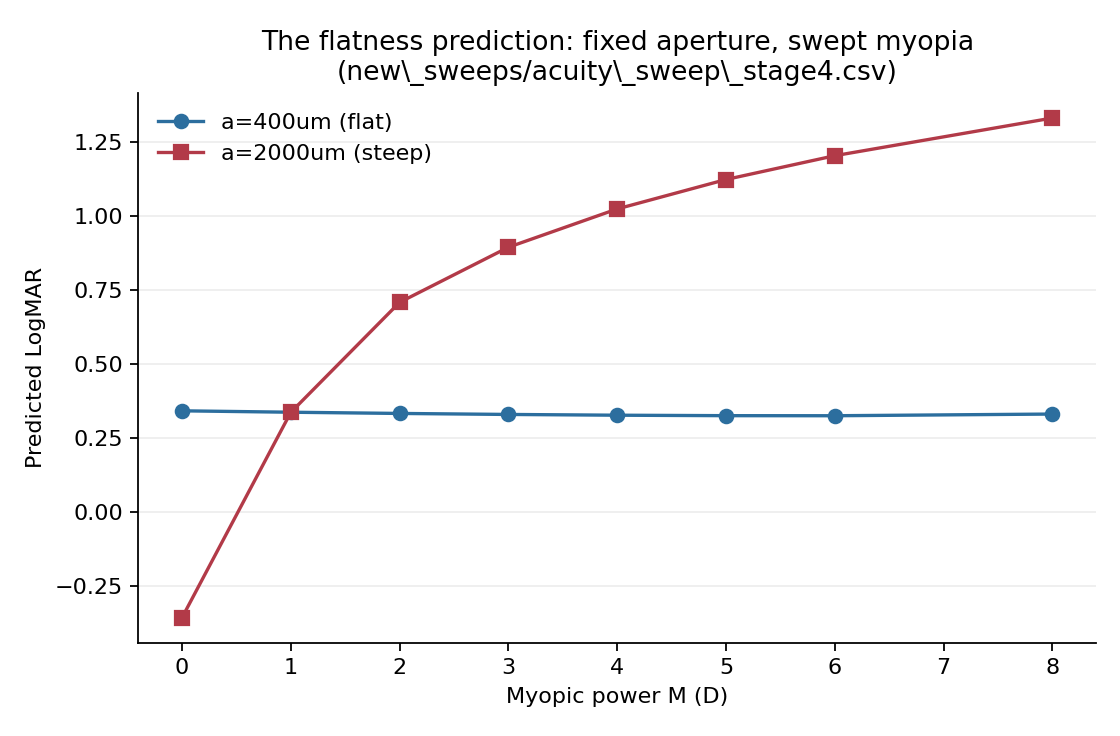
\includegraphics[width=0.75\textwidth]{figures/flatness_prediction.png}
\caption{The flatness prediction (Section~\ref{sec:flatness-prediction}): predicted
LogMAR vs.\ myopia power at fixed aperture. Recomputed directly from the current
\texttt{new\_sweeps/acuity\_sweep\_stage4.csv} (mtime 2026-09-13 00:11) for this paper;
spread at $a=400\,\mu$m is $0.0166$ LogMAR across the full 8-dioptre range, against
$1.687$ LogMAR at $a=2000\,\mu$m -- a $102\times$ difference.}
\label{fig:flatness}
\end{figure}

\section{The flatness prediction}
\label{sec:flatness-prediction}
Holding aperture fixed at $400\,\mu$m and sweeping myopia $M=0$ to $8$D, predicted
LogMAR varies by only $0.0166$ across the full range (source: this analysis, direct
computation from \texttt{new\_sweeps/acuity\_sweep\_stage4.csv}, current file) --
roughly a twentieth of one acuity-chart line, well below the $\pm0.1$ LogMAR
repeatability of human acuity testing. At this aperture, the \emph{aperture}, not the
wearer's own refractive error, sets predicted acuity. At $a=2000\,\mu$m the same sweep
spans $-0.357$ ($M=0$) to $+1.330$ ($M=8$), a spread $102\times$ larger. This is the
project's strongest, most falsifiable single prediction: it requires no knowledge of
any subject's exact prescription, only a qualitative ranking of myopia severity,
because the predicted \emph{signature} is a flat line for a well-chosen small-aperture
pinhole condition against a steep one for the unaided (or large-aperture) eye.

\section{External validation against real clinical data}
\label{sec:external-validation}
Two independently-published, directly-verified clinical datasets provide the only real
(non-simulated) LogMAR validation available anywhere in this project: Wang (2009)
\citep{wang2009} (5 apertures, $M=\{0,2,5\}$D tested, observed LogMAR
$0.28/0.31/1.00/0.40/0.50$ -- aperture-indexed only, the source paper reports
\textbf{no per-myopia-power breakdown at all}, so the same 5 observed values are
necessarily reused at every tested $M$, a real limitation of the source data, not an
approximation introduced by this project), and Kim (2017) \citep{kim2017} (single
$900\,\mu$m anchor, $N=36$, mean $M=-2.7\pm2.3$D, observed LogMAR $0.20\pm0.21$).

\subsection{A stale-data correction, made during this project's own development}
\label{sec:stale-wang}
\texttt{stage4\_human\_vision/outputs/validation\_predicted\_vs\_observed.csv} (mtime
2026-07-29 16:35) predates the 2026-08-06 \texttt{stage2/}$\to$\texttt{stage2\_fixed/}
optics fix (Section~\ref{sec:bug-shadowing}) by 8 days, and was found to give
materially different numbers from a fresh re-run with current code (e.g.\ aperture
$750\,\mu$m, $M=2$D: $0.076$ current vs.\ $1.010$ in the stale file). A corrected
``postfix'' re-run already existed
(\texttt{wang2009\_validation\_postfix\_predicted.csv}, mtime 2026-08-06 14:43) but its
own downstream calibration step had never been re-applied; this gap is closed in this
paper's own analysis (\texttt{predicted\_logmar\_analysis/wang2009\_calibration\_pooled\_stats\_postfix.csv},
computed 2026-09-28, using \texttt{stage4\_human\_vision/calibration.py}'s existing,
unmodified fitting functions). \textbf{Every number in this section uses the corrected,
post-fix data.}

\begin{table}[htbp]
\centering
\begin{tabular}{lccccc}
\toprule
Comparison & $n$ & $R^2$ & Pearson $r$ & $p$ & $R^2{>}0$ and $p{<}0.05$? \\
\midrule
$M=0$D, raw model & 5 & $-4.80$ & $-0.375$ & $0.533$ & FAIL \\
$M=2$D, raw model & 5 & $-1.41$ & $-0.180$ & $0.772$ & FAIL \\
$M=5$D, raw model & 5 & $-0.68$ & $+0.426$ & $0.474$ & FAIL \\
Pooled ($n{=}15$), raw, uncalibrated & 15 & $-2.30$ & $+0.019$ & $0.947$ & FAIL \\
Pooled, affine-calibrated, in-sample & 15 & $0.0003$ & $+0.019$ & $0.947$ & FAIL \\
Pooled, affine-calibrated, leave-one-out & 15 & $-0.31$ & $-0.928$ & $0.0000$ & FAIL \\
\bottomrule
\end{tabular}
\caption{The model fails the stated bar ($R^2>0$ AND $p<0.05$) at every single
comparison, before and after the 2026-08-06 optics fix, and before and after affine
calibration. Source: \texttt{stage4\_human\_vision/outputs/wang2009\_validation\_postfix\_stats.csv}
(per-$M$ rows) and \texttt{predicted\_logmar\_analysis/wang2009\_calibration\_pooled\_stats\_postfix.csv}
(pooled rows), both verified read directly, 2026-09-28.}
\label{tab:r2-status}
\end{table}

\begin{keybox}{The fix helped, measurably, without fixing the underlying failure}
Pooled raw $R^2$ improved from $-4.98$ (pre-fix) to $-2.30$ (post-fix) -- a real,
substantial narrowing of the gap, not a rounding-level shift -- but the model still
fails the significance bar at every single tested condition, before and after. In-sample
affine calibration gives essentially \emph{zero} explanatory power post-fix ($R^2=0.0003$,
down from $+0.132$ pre-fix), meaning the earlier apparent calibration benefit was itself
partly an artifact of the since-corrected optics bug, not a real effect of the
calibration procedure. This is reported as-is: neither ``still fails, nothing changed''
nor ``now passes,'' but the specific, quantified middle case that a real, targeted
optics fix measurably improved without resolving the underlying shortfall.
\end{keybox}

\begin{figure}[htbp]
\centering
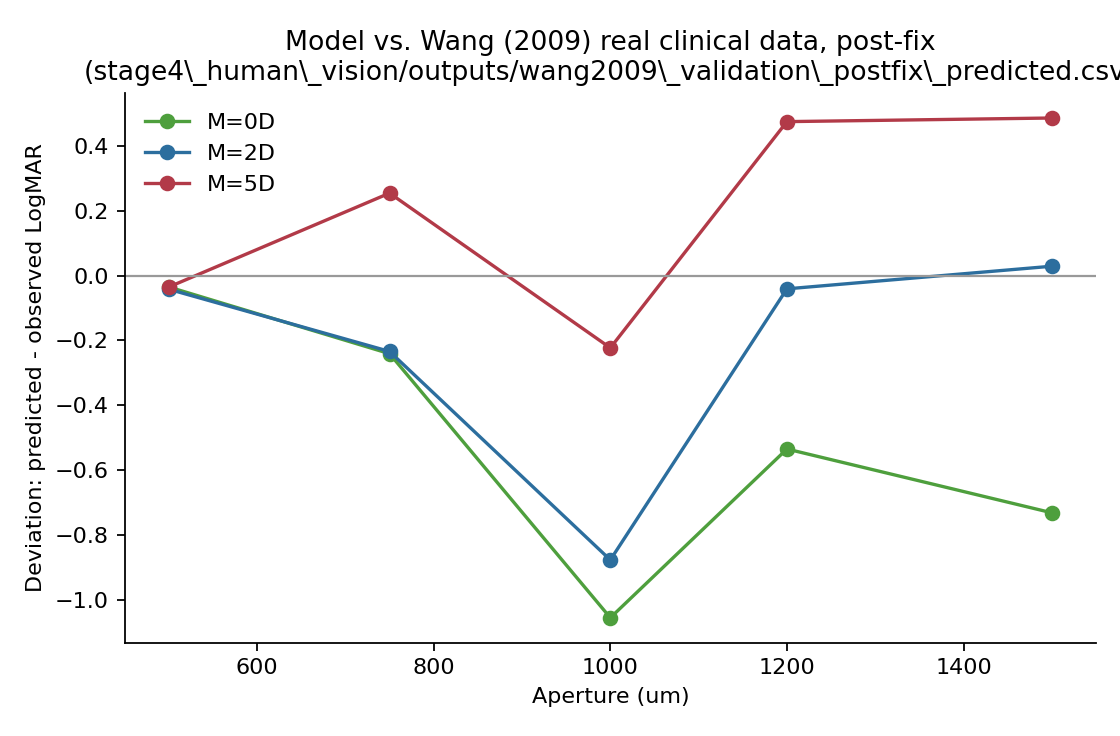
\includegraphics[width=0.75\textwidth]{figures/wang2009_deviation.png}
\caption{Model deviation (predicted $-$ observed LogMAR) vs.\ aperture, post-fix, all
three tested myopia powers. Deviation sign is not constant across the aperture range --
the model is measurably optimistic (predicts better vision than observed) at small
apertures and pessimistic at some large-aperture/high-$M$ combinations, i.e.\ this is
not a single universal bias. Source: this analysis, from
\texttt{wang2009\_validation\_postfix\_predicted.csv}.}
\label{fig:wang-deviation}
\end{figure}

\subsection{At the specific apertures this project's own array designs actually use}
Restricting the comparison to the exact (aperture, $M$) pairs the real array winners of
Chapter~\ref{ch:model-b} actually use (500 and 750\,$\mu$m, at $M=6$D and $M=2/3$D
respectively -- the only overlap between Wang's tested aperture set and this project's
own chosen apertures), the model is modestly-to-moderately \emph{optimistic}: deviation
$-0.234$ ($M=2$, $750\,\mu$m), $-0.198$ ($M=3$, $750\,\mu$m), $-0.022$ ($M=6$,
$500\,\mu$m) -- $0.2$--$2.3$ acuity-chart lines too favourable, direction consistent
across all three points (source: this analysis, from
\texttt{new\_sweeps/acuity\_sweep\_stage4.csv} cross-referenced against Wang's own
aperture-indexed observed values).

\subsection{A second real anchor: Kim (2017)}
At $a=900\,\mu$m, $M=2.7$D (this study's own reported mean): predicted LogMAR
$=0.277$, observed $0.20\pm0.21$ ($n=36$) -- deviation $+0.077$, \textbf{pessimistic},
the \emph{opposite} sign from the 500/750\,$\mu$m points above, and within one standard
deviation of the real data's own spread. This anchor was already present in this
project's own vetted literature (\texttt{stage4\_human\_vision/literature.py}, flagged
``USABLE as one additional real anchor'') but had never actually been run through the
model before this paper's own analysis. \textbf{Key honest takeaway}: the model's error
is not a single universal ``always optimistic by $X$'' bias -- both direction and
magnitude depend on the specific aperture/myopia-power region.

\subsection{A note on search-derived claims}
\label{sec:search-honesty}
A live search for additional external pinhole-aperture-vs-acuity datasets, undertaken
during this project's own development, reproduced -- verbatim -- a specific numeric
claim (``0.17 LogMAR at up to 5.5D, 1.16 LogMAR at 7--11D'') that this project's own
literature review had \emph{already} investigated and marked REJECTED after reading the
purported primary source directly and confirming those numbers do not appear anywhere
in it \citep{neuroquantology2022rejected}. This is documented here as direct, concrete
evidence that AI-search-summary claims on this specific topic are not reliable without
independent primary-source verification -- a finding this project treats as a
methodological caution for its own future literature work, not merely an isolated
incident.
